%% ABT: Automated Blue Teaming -- paper draft
%% Canonical manuscript source: paper/main.tex
%% Build from the repository root with: tectonic --outdir paper paper/main.tex
\documentclass[conference]{IEEEtran}
\usepackage{amsmath,amssymb}
\usepackage{graphicx}
\usepackage{booktabs}
\usepackage{algorithm}
\usepackage{algpseudocode}
\usepackage{hyperref}
\usepackage{xcolor}

\newcommand{\todo}[1]{\textcolor{red}{\textbf{[TODO: #1]}}}

\begin{document}

\title{ABT: An Automated Blue-Teaming Framework against Autonomous LLM-Driven Penetration Testers}

\author{
\IEEEauthorblockN{Author Names \todo{add all authors and affiliations}}
\IEEEauthorblockA{\todo{affiliation, email}}
}

\maketitle

\begin{abstract}
Autonomous, LLM-assisted penetration-testing agents such as Incalmo, APT-Agent, and
AutoHacker can plan and execute multi-host attack campaigns at a speed and scale that
manual blue teams cannot match. We present ABT (Automated Blue Teaming), a closed-loop
defence framework that (1) models the assets to protect and their required
confidentiality, integrity, availability and performance; (2) deploys host-level
Monitor-Identify-Respond (MIR) agents, analogous to an EDR; (3) controls network
topology, connectivity and service composition; (4) builds a network-wide,
two-layer Hierarchical Attack Representation Model (HARM) from topology, service and
vulnerability information and from the controls currently deployed; (5) captures the
attacker's goal (e.g., data exfiltration, privilege escalation) on this attack graph,
following Incalmo's goal abstraction; and (6) uses a master agent that plans
candidate defence actions, \emph{simulates} their effect on a copy of the network,
evaluates security, availability, performance and cost, and recommends the
highest-utility, constraint-feasible action set. We further describe how ABT ingests network specifications produced by multi-host
benchmark generators such as MHBench, and outline an iterative red-team/blue-team
procedure. The reference prototype evaluates plans on cloned network models and
measures simulated risk, service impact, cost, and SDN-policy changes; it does not
control live hosts or switches. We report a worked example on a synthetic five-host
network and specify a testbed evaluation plan.
\end{abstract}

\begin{IEEEkeywords}
automated blue teaming, attack graphs, HARM, moving target defence, autonomous red teaming, LLM pentesting agents
\end{IEEEkeywords}

\section{Introduction}
\label{sec:intro}

Large-language-model (LLM) driven red-teaming systems have recently demonstrated that
a single operator can autonomously compromise multi-host enterprise networks that
previously required a skilled human team. Incalmo~\cite{incalmo2025} separates
high-level attack \emph{planning} (performed by an LLM) from low-level
\emph{execution} (performed by deterministic expert agents for scanning, lateral
movement, information gathering and exfiltration), reporting compromise of 37 of 40
evaluated networks. APT-Agent~\cite{aptagent2026} grounds LLM decisions in an
authoritative exploit database, a failure-aware execution-state tracker, and a
HARM-based topology planner to perform verified cross-subnet pivoting with Metasploit.
AutoHacker similarly automates the pentesting kill chain end to end. Because these
systems compress what used to be days of human red-team effort into automated,
repeatable campaigns, blue teams need an equally automated, equally fast
counterpart: a system that continuously (i) knows what must be protected and to what
degree, (ii) observes hosts and the network, (iii) reconstructs the attacker's view
of the network as an attack graph, (iv) anticipates the attacker's goal, and
(v) chooses defensive actions whose benefit is verified \emph{before} deployment
rather than assumed.

This paper presents \textbf{ABT (Automated Blue Teaming)}, a framework that turns the
HARM-based security \emph{assessment} methodology of Enoch~et~al.~\cite{harmer2020,
maritime2021} into a closed-loop \emph{defence} system, and that maps assets to
concrete moving-target-defence (MTD) and conventional controls using the multi-phase,
kill-chain-indexed catalogue of MTD-in-depth~\cite{mtdindepth2026}. ABT is designed to
be attacked by, and evaluated against, the three autonomous pentesting tools above,
and to consume network specifications produced by multi-host benchmark generators such
as MHBench, which both Incalmo and APT-Agent use to build their evaluation
environments.

\textbf{Contributions.}
\begin{itemize}
\item A six-component ABT architecture (\S\ref{sec:framework}) that extends
  two-layer HARM attack graphs with an explicit attacker-goal node, a proactive and
  reactive host/network action catalogue that retains MTD, and a simulate-then-
  recommend loop with hard availability/performance constraints. An optional SDN
  control-plane emulator makes flow-rule and virtual-endpoint changes measurable.
\item A formal utility model (\S\ref{sec:utility}) combining security risk,
  legitimate-user availability, asset performance and deployment cost, used by a
  greedy marginal-utility planner.
\item A network importer (\S\ref{sec:integration}) for MHBench and APT-Agent schemas
  that maps both topologies into the common ABT model.
\item A repeated attack-observation loop (\S\ref{sec:loop}) that uses partial
  detections to trigger reactive re-planning and supports an optional proactive
  initial plan.
\item A reference, runnable implementation and a worked example on a synthetic
  five-host enterprise network (\S\ref{sec:case-study}).
\end{itemize}

\section{Related Work}
\label{sec:related}

\textbf{Attack graphs and security assessment.} HARMer~\cite{harmer2020} automates
the construction and evaluation of Hierarchical Attack Representation Models (HARMs),
two-layer attack graphs in which an upper layer captures host-level reachability and
a lower layer captures host-level exploitability as an attack tree over vulnerabilities.
Enoch~et~al.~\cite{maritime2021} extend security modelling and metrics to asset-centric
assessment of maritime vessel networks, introducing explicit protection requirements
per asset. ABT reuses the two-layer HARM construction from~\cite{harmer2020} and the
asset-centric requirement model from~\cite{maritime2021}, but drives them with a
planning and simulation loop rather than using them purely for \emph{assessment}.

\textbf{Moving target defence.} MTD-in-depth~\cite{mtdindepth2026} proposes
multi-phased MTD techniques indexed to the cyber kill chain, applying different
classes of defence (e.g., shuffling, diversity, deception) at different attack phases.
ABT adopts this phase-indexed taxonomy to tag every candidate defence action
(\S\ref{sec:actions}) so the planner can reason about kill-chain coverage per asset,
rather than treating all actions as interchangeable.

\textbf{Autonomous red teaming.} Incalmo~\cite{incalmo2025} and
APT-Agent~\cite{aptagent2026} are the two LLM-driven pentesting systems this work
targets directly; AutoHacker is treated analogously. Both Incalmo and APT-Agent are
evaluated on multi-host environments generated by MHBench, which specifies hosts,
subnets, per-host vulnerabilities (as idempotent remediation/exploit ``playbooks''),
subnet-level connectivity and exfiltration/host-access goals. APT-Agent additionally
defines its own lighter-weight topology schema (hosts, CVSS-scored service edges,
a single goal host) and vendors the HARM library of~\cite{harmer2020} for its own
path planning. \S\ref{sec:integration} describes how ABT consumes both schemas.

\section{Threat Model and Problem Statement}
\label{sec:threat-model}

We assume a defender who controls an enterprise network of hosts, each running a
known set of services with known (or estimated) vulnerabilities, connected by a
configurable topology. An external attacker --- instantiated as Incalmo, APT-Agent,
AutoHacker, or an equivalent autonomous agent --- enters through one or more
\emph{entry points} and pursues a goal $g$ such as exfiltrating data from, or gaining
a given privilege level on, a specific host (the Incalmo goal abstraction
\cite{incalmo2025}). The defender does not know the attacker's exact plan but does
know (an upper bound on) the goal space, derived from the assets being protected.
The defender's task is to choose, at each control interval, a set of actions $A$
(host-level responses via MIR agents, network-level controls, or MTD techniques)
that minimises the attacker's goal-achievement probability while respecting hard
constraints on legitimate-user availability and performance, and a cost budget.

\section{The ABT Framework}
\label{sec:framework}

\begin{figure*}[t]
  \centering
  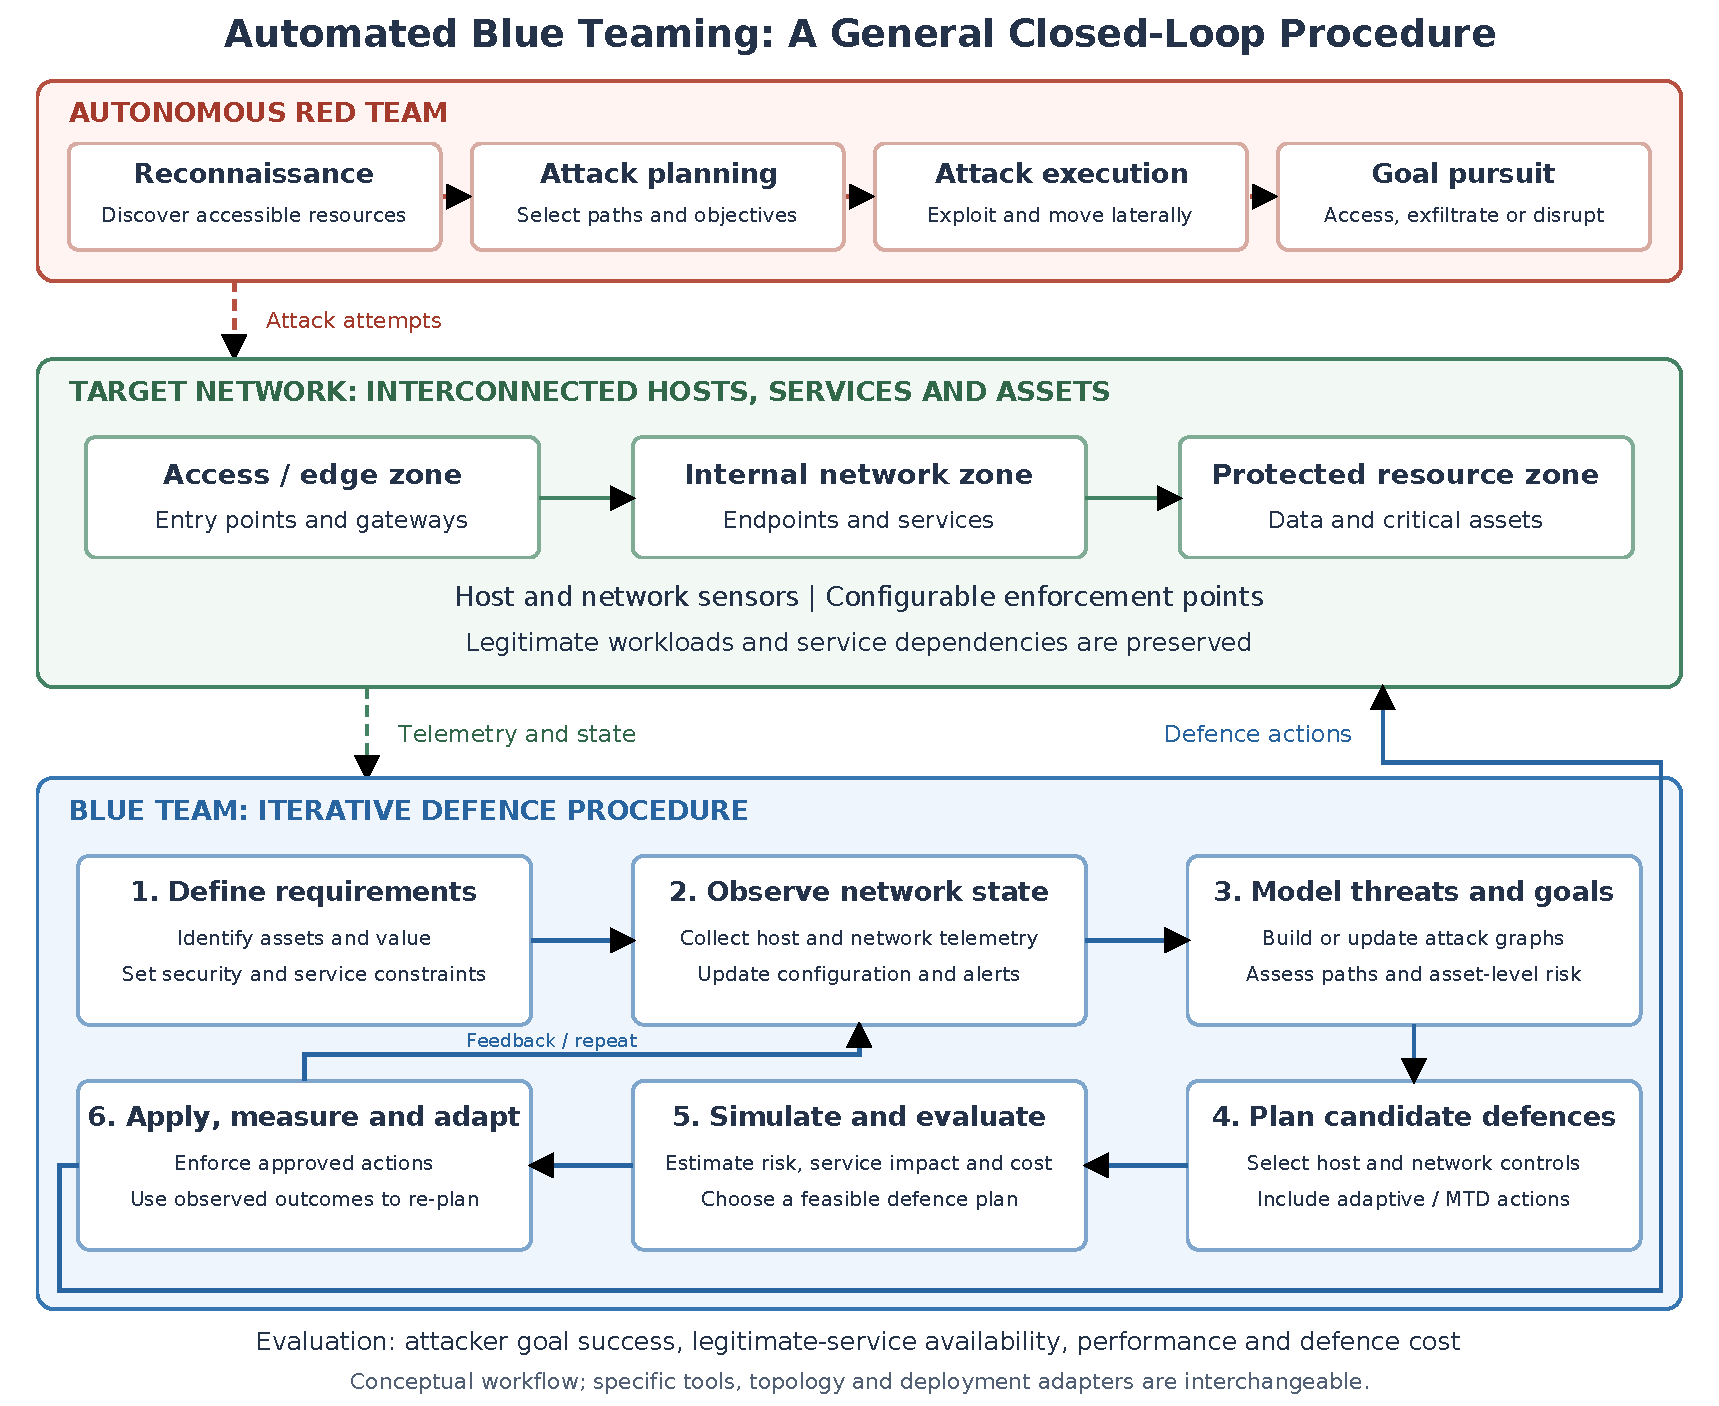
\includegraphics[width=0.96\textwidth]{abt_framework.pdf}
  \caption{General closed-loop automated blue-teaming procedure. The autonomous
  red team performs reconnaissance, planning, execution, and goal pursuit against
  an interconnected network. The blue team defines requirements, observes network
  state, models threats and goals, plans candidate controls, simulates and evaluates
  their effects, and applies approved actions. Telemetry and measured outcomes feed
  the next iteration. Zones are illustrative; the workflow is independent of a
  specific attack tool, topology, or deployment adapter. The figure describes the
  intended procedure; the current prototype simulates actions and does not actuate
  live hosts or network devices.}
  \label{fig:architecture}
\end{figure*}

Figure~\ref{fig:architecture} presents a tool-independent operational workflow.
Its six stages organise ABT's components into an iterative
observe--model--plan--evaluate--respond cycle. Host and network observations inform
the attack-graph and goal models; the planner evaluates candidate actions on a model
copy; and outcomes feed later planning. The target may contain any number of
interconnected zones, hosts, services, and protected assets rather than a fixed
topology. The figure is a conceptual workflow, not a claim that live sensors or
enforcement adapters are implemented. The following subsections give the model,
planner, and prototype details.

\subsection{Step 1 --- Asset and Protection-Requirement Model}
\label{sec:assets}

Each protected asset $a$ is defined as a tuple
\[
a = (\mathit{host}, v_a, \mathit{kind}, C, I, \alpha^{\min}_a, \pi^{\min}_a)
\]
where $v_a \ge 0$ is the business value of the asset, $\mathit{kind}\in\{\text{data},
\text{service}, \text{privilege}\}$, $C,I\in\{0,1\}$ flag whether confidentiality
and/or integrity must be preserved, $\alpha^{\min}_a\in[0,1]$ is the minimum share of
legitimate traffic touching $\mathit{host}$ that must still succeed, and
$\pi^{\min}_a\in[0,1]$ is the minimum acceptable performance factor of
$\mathit{host}$. Legitimate workloads are modelled as weighted flows
$f=(\mathit{src},\mathit{dst},\mathit{port},w_f)$ that the defender must not
needlessly break. This directly generalises the asset-centric model
of~\cite{maritime2021} with explicit availability/performance SLOs.

\subsection{Step 2 --- MIR Agents (Host Level)}
\label{sec:mir}

A \emph{Monitor-Identify-Respond} (MIR) agent, analogous to an EDR, is deployed per
host. It (i) \emph{monitors} process, network and authentication events; (ii)
\emph{identifies} indicators of compromise and raises alerts that update the master
agent's belief about which hosts are compromised (\S\ref{sec:loop}); and (iii)
\emph{responds} by executing host-level actions issued by the master agent: patching
a specific vulnerability, disabling a service, enabling software diversity, or
isolating the host from the network.

\subsection{Step 3 --- Network-Level Control}
\label{sec:netctl}

A network controller enforces the topology: which flows $(\mathit{src},
\mathit{dst},\mathit{port})$ are permitted, which services are exposed at each
entry point, and which hosts belong to which network segment. It also executes
network-level MTD actions, notably IP/port shuffling, which the planner may select
independently of host-level MIR actions.

MTD does not inherently require SDN: address or port changes can also be coordinated
through host firewalls, DHCP/DNS, virtual-machine or container networking, and
network-address translation. These alternatives need their own coordination and
deployment mechanisms. For the initial network-control study, we use an explicitly
simulated SDN control plane to make flow-rule updates and virtual-endpoint remapping
observable and repeatable. ABT's \texttt{SDNController} model stores virtual-IP leases,
blocked flows, and policy-update counts; candidate rules and shuffles are applied to
a cloned network for preview, and only the selected plan mutates the in-memory
network. This is an SDN control-plane emulation, not integration with a live
controller. The same planner remains applicable without SDN when supplied with a
different network-controller adapter.

\textbf{Non-MTD network controls.} Enterprise network guidance treats segmentation,
firewall policy, monitoring, and resource-level access control as complementary
controls rather than relying on a single perimeter~\cite{nist800215,nist80041r1}.
ABT's current network model directly represents permitted host-to-host flows; its
implemented network actions are flow blocking and coarse host isolation. Candidate
extensions include least-privilege segmentation, directional egress filtering,
protective DNS, network traffic analysis, and graduated quarantine. Their
operational mechanisms and deployment prerequisites differ, so this paper selects a
small implementable subset rather than assuming that every control can be represented
by deleting a graph edge.

\textbf{Host controls.} Host-level candidates include vulnerability patching,
disabling an unnecessary service, host-firewall policy, application execution
controls, credential hardening, and endpoint isolation. The current prototype
simulates patching, disabling a service, MIR deployment, and host isolation; it does
not invoke package managers, service managers, endpoint agents, or host-firewall
APIs. NIST's control catalogue includes system monitoring, malicious-code
protection, and flaw remediation as distinct control functions~\cite{nist80053}.
Their actuator and operational risk are also distinct: patching needs a
platform/package mapping and compatibility checks; disabling a service can interrupt
a legitimate dependency; host isolation can sever management and recovery access.
We therefore distinguish simulator support from deployable integration.

\textbf{Proactive and reactive controls.} We call a control \emph{proactive} when it
is installed or planned before an attack alert, and \emph{reactive} when an observed
event triggers a response. This is an operational distinction, not an intrinsic
property of the technique: for example, an ACL may be a proactive baseline or a
reactive containment rule, and MTD may be scheduled proactively or triggered by
telemetry. We retain the existing MTD actions (software diversity and IP/port
shuffling) as a separate control family and baseline; they are not replaced by the
non-MTD portfolio. The proposed portfolio and feasibility assessment are in
\S\ref{sec:portfolio}.

\textbf{Deferred network controls.} Protective DNS can block, redirect/sinkhole, and
alert on matching queries~\cite{cisapdns,d3fenddns}, but ABT first needs domain-query
state and a model for direct-IP connections. Network traffic analysis is
observational evidence, not itself inline blocking~\cite{d3fendnta}; live sensors,
false-positive rates, and alert delays would need to be integrated. ZTNA requires
identity/device context and policy-enforcement points absent from the current
flow-only model~\cite{nist800207,cisaztmm}. Rate limiting requires traffic demand,
link capacity, latency, and throughput state. We defer these controls from the
initial implementation and deployment subset.

Zero-trust network access is a longer-term extension rather than a flow-only
action: per-request access decisions require identity, device/context attributes,
and policy-enforcement points that the present ABT model does not
represent~\cite{nist800207,cisaztmm}. Similarly, rate limiting requires traffic
demand, link capacity, latency, and throughput state, which are absent from the
current binary connectivity model. We therefore defer both until those state
variables and their operational costs can be evaluated.

\subsection{Step 4 --- Network-Wide Attack Graph (Two-Layer HARM)}
\label{sec:harm}

Following~\cite{harmer2020}, ABT builds a two-layer HARM from the current topology,
service inventory, known vulnerabilities, and currently deployed controls.

\textbf{Lower layer (per-host attack tree).} For host $h$ and service port $p$ with
installed vulnerabilities $\{v_1,\dots,v_k\}$, each $v_i$ having exploit-success
probability $p_i$ and required minimum privilege $\mathit{priv}_i$, the probability
that an attacker requiring at least privilege $\mu$ successfully exploits the service
is a noisy-OR over applicable vulnerabilities, scaled by a host-level defence factor
$\phi(h)$:
\begin{align}
P_{\mathrm{host}}(h,p,\mu) &= \Big(1-\!\!\!\prod_{i:\ \mathit{priv}_i\ge\mu}\!\!\!(1-p_i)\Big)\cdot\phi(h) \label{eq:hostp}\\
\phi(h) &= (1-\beta_{\mathrm{MIR}})^{\mathbb{1}[\mathrm{mir}_h]}\cdot
            \beta_{\mathrm{div}}^{\mathbb{1}[\mathrm{div}_h]}\cdot
            \beta_{\mathrm{shuf}}^{\mathbb{1}[\mathrm{shuf}_h]} \label{eq:phi}
\end{align}
where $\beta_{\mathrm{MIR}}$, $\beta_{\mathrm{div}}$, $\beta_{\mathrm{shuf}}\in[0,1]$
are the (empirically calibrated) probabilities that an installed MIR agent,
software-diversity control, or IP/port-shuffling control respectively blocks the
exploitation step.

\textbf{Upper layer (host reachability graph).} For permitted flows between hosts
$s$ and $d$, the edge success probability is the noisy-OR of
$P_{\mathrm{host}}(d,p,\mu)$ over all ports $p$ reachable from $s$ to $d$:
\[
P_{\mathrm{edge}}(s,d,\mu) = 1-\prod_{p:\,(s,d,p)\in F} \big(1-P_{\mathrm{host}}(d,p,\mu)\big)
\]
where $F$ is the current set of permitted flows (including attacker-to-entry-point
flows). Given a goal $g=(\mathit{kind}, h_g, \mu_g, \mathit{asset})$, ABT enumerates
simple paths from every entry point (and from every host already believed
compromised, \S\ref{sec:loop}) to $h_g$ by depth-first search, computing each path's
attack success probability (ASP) as the product of its edge probabilities, with the
final edge evaluated at privilege $\mu_g$. The overall goal-achievement probability
is the noisy-OR over the $k$ most probable paths returned:
\[
P(g) = 1-\prod_{\text{path}\in\mathrm{paths}(g)}(1-\mathrm{ASP}(\text{path}))
\]

\subsection{Step 5 --- Goal Capture}
\label{sec:goal}

ABT represents the attacker's objective using Incalmo's goal
abstraction~\cite{incalmo2025}: a target host, a kind
(\emph{exfiltrate}/\emph{escalate}/\emph{disrupt}), a minimum privilege level, and
optionally a named asset. This lets the same attack-graph machinery
(\S\ref{sec:harm}) serve both data-exfiltration goals (as in MHBench's
\texttt{data\_exfiltration} goal type) and escalation/host-access goals, and lets the
risk metric (\S\ref{sec:utility}) be computed per goal and aggregated by asset value.

\subsection{Step 6 --- Master Agent: Plan, Simulate, Evaluate, Recommend}
\label{sec:master}

The master agent maintains the current world model (topology, services,
vulnerabilities, deployed controls, and the set of hosts believed compromised from
MIR alerts), enumerates a pool of candidate actions
(\S\ref{sec:actions}), and greedily searches for the action set with highest utility
(\S\ref{sec:utility}) subject to hard constraints, \emph{simulating} every candidate
on a private copy of the network before evaluating it so the live network is never
perturbed by an infeasible or low-value trial.

\subsection{Defence Action Catalogue}
\label{sec:actions}

Table~\ref{tab:actions} retains the existing MTD and conventional host/network
actions. The proactive/reactive classification describes their intended trigger in
the proposed experiment; it does not assert that live deployment adapters exist.

\begin{table}[t]
\centering
\small
\setlength{\tabcolsep}{2pt}
\caption{Existing simulated action catalogue, retained MTD controls, and intended
operational timing. Live actuation is not implemented.}
\label{tab:actions}
\begin{tabular}{@{}p{0.26\columnwidth}p{0.13\columnwidth}p{0.17\columnwidth}p{0.28\columnwidth}@{}}
\toprule
Action & Level & Timing & Implementation status \\
\midrule
MIR telemetry / response & host & Both & Simulated event ingestion; no real sensor/agent \\
Patch vulnerability & host & Proactive & Removes modeled CVE; no package backend \\
Disable service & host & Proactive & Simulated service state; no service-manager backend \\
Isolate host & host & Reactive & Coarse flow removal; no recovery-channel semantics \\
Software diversification (MTD) & host & Proactive* & Existing simulated MTD action \\
IP/port shuffling (MTD) & network & Proactive* & Existing simulated MTD action \\
Segmentation / flow block & network & Proactive / reactive & Flow / SDN-state mutation simulated; live controller adapter absent \\
\bottomrule
\end{tabular}
\end{table}

\noindent *MTD actions remain in the action catalogue. A future telemetry-triggered
MTD policy may also use them reactively; the initial comparison treats them as
proactive controls.

\subsection{Selected Defense Portfolio and Deployment Feasibility}
\label{sec:portfolio}

We select the initial portfolio by asking whether a control (i) can be represented
with the present model or a small extension, (ii) has a plausible enforcement point
in an isolated benchmark, (iii) can be rolled back and tested without disrupting
production, and (iv) has an outcome measurable with current ABT metrics. This
selection keeps MTD and adds a bounded host/network subset. Table~\ref{tab:portfolio}
separates \emph{simulator feasibility} from \emph{deployment feasibility}; passing
the former does not imply a production-ready controller.

\begin{table}[t]
\centering
\small
\setlength{\tabcolsep}{2pt}
\caption{Selected initial portfolio and deferred alternatives. The prototype's
action effects are simulator mutations; deployment requires separate adapters.}
\label{tab:portfolio}
\begin{tabular}{@{}p{0.19\columnwidth}p{0.12\columnwidth}p{0.31\columnwidth}p{0.28\columnwidth}@{}}
\toprule
Control & Choice & Model / testbed path & Caveat \\
\midrule
Proactive network segmentation & Select & Least-privilege rules over declared service and legitimate flows; Mininet/OVS target. & Add rule precedence, dry-run, read-back, and rollback. \\
Reactive network flow block & Select & Block one attacker-relevant flow after a confirmed/injected alert; same OVS policy path. & Preserve recovery and legitimate flows; log every update. \\
Proactive host patch / disable & Select for simulation & Existing actions; allowlisted Ansible tasks on disposable Linux hosts. & No generic CVE-to-package mapping or live patching. \\
Reactive host quarantine & Select for simulation & Existing action; host-firewall/EDR profile is the deployment target. & Refine all-flow isolation to retain recovery access. \\
MTD (diversity, shuffle) & Retain & Existing MTD actions remain a separate, proactive baseline. & Effects simulated; probabilities uncalibrated. \\
DNS / NTA sensors & Defer & Requires resolver integration, domain state, and sensor events. & False positives and detection delay not modeled. \\
ZTNA / rate limit / allowlist & Defer & Requires identity, traffic-load, or app-policy state. & Larger model and platform-specific validation. \\
\bottomrule
\end{tabular}
\end{table}

For deployment planning, we target an isolated Linux testbed first, rather than
claiming cross-platform or production support. Docker can provide reproducible
containerized endpoints and service topologies, but its built-in network drivers
alone do not provide an OpenFlow-controlled switch or SDN controller
\cite{dockernetworking}. Docker is therefore suitable for endpoint and
container-network adapter tests, not by itself for validating SDN flow-rule
behaviour. For the SDN experiment, we select Mininet with Open vSwitch (OVS) and an
OpenFlow controller: Mininet provides virtual hosts and switches for SDN
experiments, while OVS supports programmable OpenFlow switching
\cite{mininet,openvswitch}. Docker containers may optionally provide test services
if attached through a Linux-host OVS integration; they are not required for the
initial topology. The prototype's SDN controller remains an emulator until this
adapter is implemented and validated.

The network adapter would translate an approved abstract policy into testbed flow
rules; host tasks would use restricted configuration-management playbooks. Each
adapter must support dry-run, explicit approval, pre-change snapshot, post-change
read-back, health checks, and rollback. We will run the testbed in an isolated
Linux host or VM; Docker Desktop on macOS is not the target enforcement environment
for kernel/OVS-level measurements. Windows hosts, heterogeneous production
networks, direct autonomous actuation, and external DNS/IDS services are outside
this initial deployment target. NIST firewall guidance and CISA incident response playbooks motivate policy review,
containment, and recovery planning, not the assumption that ABT already implements
those integrations~\cite{nist80041r1,cisairplaybook}. For a Linux firewall
alternative, nftables supports atomic ruleset replacement; this is distinct from
the selected OpenFlow/OVS experiment. Windows firewall deployment is possible
through centrally managed Group Policy, but is outside the initial Linux-only
target~\cite{nftablesatomic,windowsfirewallgpo}.

The deployment path is staged: first validate endpoint services and the abstract
policy adapter with containers; then validate dynamic flow installation, packet
reachability, and policy-update effects in Mininet/OVS. Docker-only results will be
reported as container-network tests, not as SDN results. Neither stage changes the
current simulator's status or implies live deployment has already been completed.

The experimental protocol separates two conditions: (1) \emph{proactive}, where
the planner applies baseline segmentation and selected host hardening before the
first attack round; and (2) \emph{reactive}, where a telemetry/attack-result event
triggers a flow block and/or host quarantine followed by replanning. MTD remains
available in both comparisons as its own action family; it is neither removed nor
relabelled as a conventional firewall control. Report effect per mode and ablate
proactive-only, reactive-only, MTD-only, non-MTD-only, and combined portfolios.

\todo{Re-derive this table directly from the MTD-in-depth~\cite{mtdindepth2026}
technique taxonomy rather than from our current assumption; extend with
credential rotation, decoys/honeytokens, and data-at-rest encryption for the
\emph{objective} phase.}

\section{Utility Model and Planning}
\label{sec:utility}

For a candidate action set $A$ applied to a simulated copy of the network, ABT
computes:
\begin{align}
\mathrm{risk}(A) &= \frac{\sum_{g\in G} v_{a(g)}\, P_A(g)}{\sum_{g\in G} v_{a(g)}} \\
\mathrm{avail}(A) &= \frac{\sum_{a\in \mathrm{Assets}} v_a\cdot\mathrm{avail}_a(A)}{\sum_{a} v_a}\\
\mathrm{avail}_a(A) &= \frac{\sum_{f\in L_a} w_f\cdot\mathbb{1}[f\ \text{works}]}{\sum_{f\in L_a} w_f}\\
\mathrm{perf}(A) &= \frac{\sum_{a} v_a\cdot\big(1-o_a(A)\big)}{\sum_a v_a}\\
\mathrm{cost}(A) &= \sum_{\alpha\in A} c_\alpha
\end{align}
where $G$ is the set of attacker goals, $v_{a(g)}$ the value of the asset targeted by
goal $g$, $L_a$ the legitimate flows touching asset $a$'s host, and $o_a(A)$ the
cumulative performance overhead (from installed MIR agents, diversity, shuffling,
and patch downtime) on $a$'s host. The overall utility is
\begin{equation}
\begin{aligned}
U(A) ={}& w_s\big(1-\mathrm{risk}(A)\big) + w_a\,\mathrm{avail}(A)\\
       &+ w_p\,\mathrm{perf}(A)
       - w_c\min\!\Big(1,\tfrac{\mathrm{cost}(A)}{B}\Big)
\end{aligned}
\label{eq:utility}
\end{equation}
subject to the hard constraints $\mathrm{avail}_a(A)\ge\alpha^{\min}_a$,
$1-o_a(A)\ge\pi^{\min}_a$ for every asset $a$, and $\mathrm{cost}(A)\le B$ for budget
$B$. ABT's reference planner (Algorithm~\ref{alg:planner}) is a greedy, anytime
marginal-utility search: at each step it simulates every unused candidate action in
combination with the current set, keeps the one with the largest utility gain that
remains feasible, and stops when no action improves utility or a cap on plan size is
reached. \todo{compare against an ILP/ MCTS/ beam-search planner and report
optimality gap on small networks, as proposed in the evaluation protocol.}

\begin{algorithm}[t]
\caption{Greedy marginal-utility defence planning}
\label{alg:planner}
\begin{algorithmic}[1]
\Require network $N$, goals $G$, weights $w$, budget $B$, max actions $m$
\State $A \gets \emptyset$; $u \gets U_N(\emptyset)$ \Comment{baseline utility}
\For{$i=1$ \textbf{to} $m$}
  \State $\alpha^\star \gets \mathrm{None}$; $\Delta^\star \gets 0$
  \For{each candidate action $\alpha \notin A$}
    \State $N' \gets \mathrm{simulate}(N, A\cup\{\alpha\})$
    \If{$N'$ violates a hard constraint} \textbf{continue} \EndIf
    \State $\Delta \gets U(N') - u$
    \If{$\Delta > \Delta^\star$} $\alpha^\star \gets \alpha$; $\Delta^\star\gets\Delta$ \EndIf
  \EndFor
  \If{$\alpha^\star = \mathrm{None}$} \textbf{break} \EndIf
  \State $A \gets A \cup \{\alpha^\star\}$; $u \gets u + \Delta^\star$
\EndFor
\State \Return $A$
\end{algorithmic}
\end{algorithm}

\section{Integrating Multi-Host Network Benchmarks}
\label{sec:integration}

To avoid re-authoring target networks by hand, ABT defines an import layer that maps
the schemas used by the benchmark generators consumed by Incalmo and APT-Agent into
the common network model of \S\ref{sec:assets}--\S\ref{sec:harm}.

\textbf{MHBench.} MHBench-generated environments specify, per subnet, a list of hosts
with per-host \emph{vulnerability playbooks} (typed as \texttt{lateral\_movement} or
\texttt{privilege\_escalation}, each naming an Ansible playbook rather than a CVE/port),
subnet-level connectivity, and goals of type \texttt{data\_exfiltration} or
\texttt{host\_access} with a target host/user. ABT's importer (i) creates one
\texttt{Host} per MHBench host; (ii) synthesises a \texttt{Service}/\texttt{Vuln} pair
per distinct vulnerability playbook on a host, since MHBench does not assign ports or
exploit probabilities explicitly \todo{calibrate default $p$ and impact per playbook
type from MHBench's own experiment logs rather than using a flat default}; (iii)
expands subnet-to-subnet connectivity into host-level flows and adds the explicit
\texttt{from\_host\_ip}$\to$\texttt{to\_host\_ip} edges recorded on each vulnerability;
(iv) marks external subnets as entry points; and (v) converts each MHBench goal into
an ABT \texttt{AttackGoal} and a corresponding \texttt{Asset}.

\textbf{APT-Agent topology schema.} APT-Agent's own (lighter) topology format lists
hosts by IP with a role label and edges annotated with port, service, CVSS score and
Metasploit exploit module, plus an optional \texttt{pivot\_network} for
internal/lateral edges, and a single goal host. This maps almost directly onto ABT's
\texttt{Host}/\texttt{Service}/\texttt{Vuln}/flow model, with exploit probability
derived from the CVSS score (\todo{validate this mapping; CVSS base score is not a
calibrated exploit-success probability}) and the goal host converted to a single
\texttt{AttackGoal}.

Because both importers target the same \texttt{Network} model, every downstream ABT
component (HARM construction, action catalogue, planner, simulator) is reused
unmodified regardless of which generator produced the target environment.

\section{Closing the Loop with Attack Execution}
\label{sec:loop}

To test that the defence actually adapts to observed attacker behaviour rather than
only to a static model, ABT supports a multi-round \emph{training/validation loop}
against a red-team adapter (a thin interface implemented, in the reference tool, for
Incalmo, APT-Agent and AutoHacker, and for a Monte-Carlo stand-in used for fast,
offline validation). The loop can optionally apply an initial proactive plan before
the first attack; the current candidate-action catalogue supports host patching,
service disabling, MIR installation, and the retained MTD actions, while the
segmentation policy extension remains future work. In round $t$: (1) the attacker
attempts its goal(s) against the current network state, returning not only
success/failure but the path of hosts it
traversed; (2) on success, each host on that path (excluding the goal host itself) is
marked compromised with detection probability $p_{\mathrm{det}}$, modelling imperfect
MIR detection, and reported to the master agent; (3) the master agent re-plans
(Algorithm~\ref{alg:planner}) using the updated, partially-compromised world model and
executes the resulting actions; (4) risk, availability, performance and the
attacker's per-round and cumulative realised success rates are logged for round $t$.
The reference implementation stops early after a configurable number of consecutive
rounds with neither newly detected hosts nor defence actions. Repeating this for $T$
rounds lets us measure both the \emph{convergence rate} (how many rounds until the
defence state stabilises) and the \emph{residual risk} after convergence, separately
for each red-team tool, which we propose as the core quantitative result of the full
paper (\S\ref{sec:evaluation}).

\section{Worked Example}
\label{sec:case-study}

\begin{table}[t]
\centering
\caption{Single-shot planning result on a synthetic 5-host enterprise network
(web/DMZ entry point, app server, database, file server, AD/LDAP), evaluated against
Monte-Carlo stand-ins for Incalmo and APT-Agent with persistence 4 and 2 respectively.}
\label{tab:casestudy}
\begin{tabular}{@{}lrr@{}}
\toprule
Metric & Before plan & After plan \\
\midrule
Risk (value-weighted $P(g)$) & 0.468 & 0.000 \\
Legitimate-user availability & 1.00 & 1.00 \\
Asset performance factor & 1.00 & 0.99 \\
Utility (Eq.~\ref{eq:utility}) & 0.666 & 0.856 \\
Incalmo-stub success rate & 0.72 & 0.00 \\
APT-Agent-stub success rate & 0.72 & 0.00 \\
\bottomrule
\end{tabular}
\end{table}

As a proof of concept, we ran the reference implementation on a hand-built
five-host network (Table~\ref{tab:casestudy}). The planner selected five actions:
installing MIR agents on the two hosts on the highest-ASP paths, disabling two
unused services, and patching one application vulnerability, for a total cost of
5.0 against a budget of 12.0. \todo{replace this illustrative example with
results on an MHBench-generated environment (\S\ref{sec:integration}) and the
multi-round loop (\S\ref{sec:loop}) once both are implemented and validated against
the real Incalmo/APT-Agent tools rather than the Monte-Carlo stand-ins.}

\section{Evaluation Plan}
\label{sec:evaluation}

We propose to answer the following research questions on MHBench-generated
Equifax-like, ICS, and enterprise topologies of increasing size (10--1000 hosts):
the simulator is the current implementation baseline. A separate isolated Linux
Mininet/OVS testbed is the planned environment for validating actual flow-rule
enforcement; Docker is optional for hosting endpoints and is not treated as an
OpenFlow datapath. Results from the two environments will be reported separately.
In Mininet/OVS runs, record rule-installation and removal latency, packet loss,
reachability of required and prohibited flows, and service latency/throughput before
and after each policy update; Docker-only runs report container-network results and
must not be presented as OpenFlow measurements.

\begin{description}
\item[RQ1 (effectiveness)] How much does ABT reduce goal-achievement probability
  and realised attacker success rate against Incalmo, APT-Agent, and AutoHacker,
  compared to no defence and to a static (non-adaptive) defence baseline?
\item[RQ2 (cost to legitimate users)] What is the availability and performance
  impact of ABT's recommended plans on legitimate workloads, and how does this
  trade off against RQ1 as the utility weights $w_s,w_a,w_p,w_c$ vary?
\item[RQ3 (planner quality and scalability)] How close is the greedy planner to an
  optimal (ILP/exhaustive) plan on small networks, and how does planning latency
  scale with network size?
\item[RQ4 (adaptivity)] How many attack rounds (\S\ref{sec:loop}) does ABT need to
  converge to a low-risk configuration for each red-team tool, and what is the
  residual risk at convergence? Compare a proactive-only initial plan with
  alert-triggered reactive re-planning, and ablate host-only, network-only, MTD-only,
  non-MTD-only, and combined actions, as well as simulation-guided vs. unguided
  (apply-first) planning.
\end{description}

\section{Discussion and Limitations}
\label{sec:limitations}

The HARM path-probability model (\S\ref{sec:harm}) treats paths as independent,
which overestimates risk when paths share hops; a shared-hop-aware aggregation (e.g.,
inclusion--exclusion on a bounded path set, or exact computation on the DAG) is left
for future work. The host-level defence factors
$\beta_{\mathrm{MIR}},\beta_{\mathrm{div}},\beta_{\mathrm{shuf}}$ and the MHBench
playbook-to-probability mapping (\S\ref{sec:integration}) are currently placeholders
and must be calibrated against real red-team runs rather than assumed. The MIR agent
and network controller are, in the current reference implementation, model mutations
rather than real enforcement points (e.g., \texttt{iptables}/SDN/cloud security
groups); a production deployment requires a signed command channel from the master
agent to real hosts and network devices, and a human-approval gate before autonomous
actions are applied outside of simulation, which we treat as an explicit design
requirement rather than an afterthought. Finally, the current learning loop
(\S\ref{sec:loop}) models \emph{our} adaptation to the attacker but not the
attacker's adaptation to \emph{us}; evaluating against the real Incalmo/APT-Agent
agents (which can themselves replan) rather than Monte-Carlo stand-ins is necessary
to validate this interaction.

\section{Conclusion}
\label{sec:conclusion}

We presented ABT, a six-step automated blue-teaming framework that extends HARM-based
security assessment~\cite{harmer2020,maritime2021} and kill-chain-indexed moving
target defence~\cite{mtdindepth2026} into a closed-loop planner that simulates,
evaluates and recommends defence actions against autonomous LLM-driven pentesting
agents~\cite{incalmo2025,aptagent2026}. We described how ABT imports MHBench- and
APT-Agent-style network specifications into a common model and how it closes the
loop with repeated attack execution. \todo{finalise once the importer, the learning
loop and the full evaluation (\S\ref{sec:evaluation}) are implemented and run against
the real red-team tools.}

\bibliographystyle{IEEEtran}
{\sloppy
\bibliography{refs}
}

\end{document}
